\chapter{ML}

\section{Artificial neuron}

Artificial neurons, also called perceptrons were developed in the late 1950s and early 1960s, firstly introduced by Rosenblatt in his paper \textbf{TODO}\footnote{\url{http://citeseerx.ist.psu.edu/viewdoc/download?doi=10.1.1.335.3398&rep=rep1&type=pdf}}. His idea was to develop a model capable of simulating the activities present in the human brain cell, in order to create artificial intelligence. As it turned out, simulating the brain using such a simple model as the perceptron is impossible. However, later research discovered a considerable potential in the field of classification and regression, which lead to design of modern artificial neural networks as we know them today.

Perceptron is a simple probabilistic model, which takes several weighted real inputs and produces one real output.

\vspace{3mm}

\begin{minipage}[c]{0.35\textwidth}
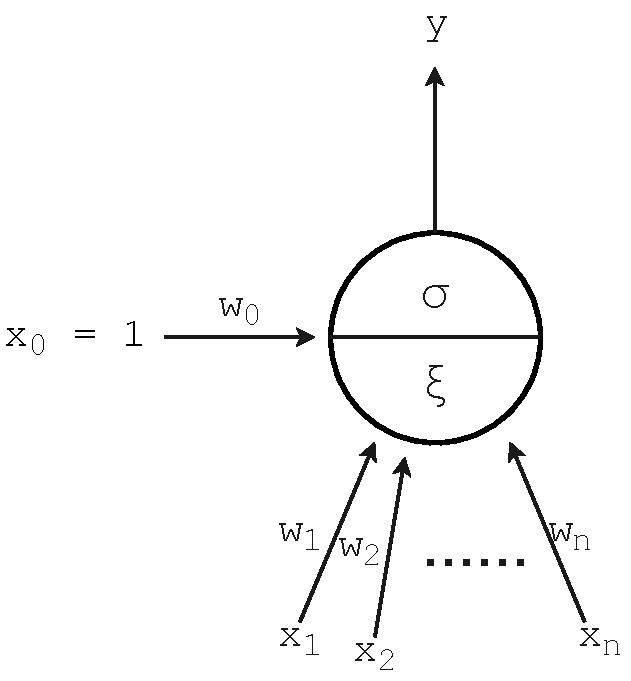
\includegraphics[width=\textwidth]{tex/images/perceptron}
\end{minipage}
\hfill
\begin{minipage}[c]{0.55\textwidth}


\begin{itemize}

\item \textbf{TODO} <---- figure caption 
\item $x_1, \cdots, x_n$ are real \textbf{inputs}
\item $x_0$ is always equal to 1
\item $w_0, w_1, \cdots, w_n$ are real \textbf{weights}
\item $\xi$ is inner \textbf{potential}, \\$\xi = w_0 + \Sigma_{i=1}^n w_i x_i$
\item $y$ is real \textbf{output} given as $y = \sigma(\xi)$
\item $\sigma$ is an \textbf{activation function}

\end{itemize}
\end{minipage}

\section{activation}

An activation function $\sigma: \mathbb{R} \rightarrow \mathbb{R}$ is applied to the inner potential $\xi$, and it defines the output value of perceptron. It introduces a powerful tool into machine learning, and that is \textbf{non-linearity}. Without the activation, the potential by itself is a simple polynomial of a degree of one. That would limit the learning ability of the neural network into being a simple regression model. However, using different activation function, we can adapt the model to more complicated mappings.

\begin{figure}[h]

\centering
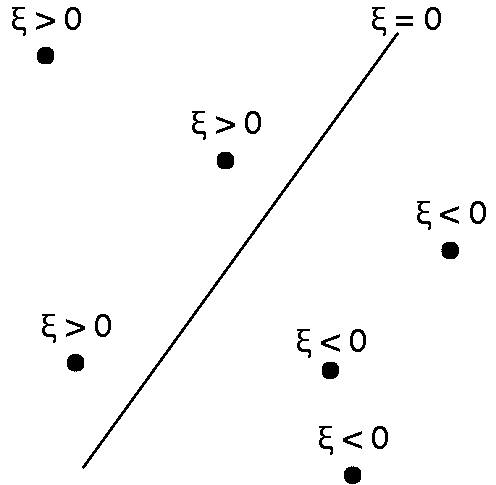
\includegraphics[width=0.5\textwidth]{tex/images/activation-vis}
\caption{Visualization of an activation function $\sigma(\xi) = 1$ for $\xi \geq 0$ and $\sigma(\xi) = 0$ for $\xi < 0$, which defines a separation hyperplane in n-dimensional space.}
\end{figure}

Some desirable properties of an activation function include \textbf{TODO}\footnote{\url{https://en.wikipedia.org/wiki/Activation_function\#Comparison_of_activation_functions}}

\begin{itemize}

\item \textit{non-linearity} - in order to map more complex functions (allows universal function approximations)
\item \textit{continuous differentiability} - necessity for gradient-based optimization methods
\item \textit{range} - for infinite range, training is generally more efficient
\item \textit{monotonicity} - the error surface associated with a single-layer models is guaranteed to be convex
\item \textit{approximates identity near the origin} - initial weights can be randomized with small differences around the origin

\end{itemize}

Here are some examples of activation functions:

\textbf{TODO} - cite \url{https://towardsdatascience.com/activation-functions-and-its-types-which-is-better-a9a5310cc8f}

\begin{tabular}{| p{25mm} | c | l | l |}

\hline

Name & Plot & Equation & Description \\

\hline

Identity & \begin{minipage}{.2\textwidth}
      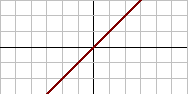
\includegraphics[width=\textwidth]{tex/images/activation/identity}
    \end{minipage} & $f(x) = x$ & - \\
      
Binary step & \begin{minipage}{.2\textwidth}
      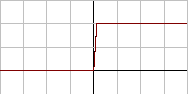
\includegraphics[width=\textwidth]{tex/images/activation/binstep}
    \end{minipage} & - & -  \\
    
Sigmoid & \begin{minipage}{.2\textwidth}
      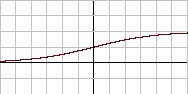
\includegraphics[width=\textwidth]{tex/images/activation/sigmoid}
    \end{minipage} & - & - \\

tanh & \begin{minipage}{.2\textwidth}
      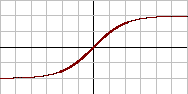
\includegraphics[width=\textwidth]{tex/images/activation/tanh}
    \end{minipage} & - & - \\
    
ReLU & \begin{minipage}{.2\textwidth}
      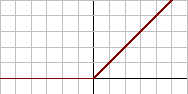
\includegraphics[width=\textwidth]{tex/images/activation/relu}
    \end{minipage} & - & - \\
    
Leaky ReLU & \begin{minipage}{.2\textwidth}
      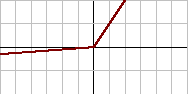
\includegraphics[width=\textwidth]{tex/images/activation/lrelu}
    \end{minipage} & - & -\\
    
Randomized \newline Leaky ReLU & \begin{minipage}{.2\textwidth}
      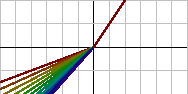
\includegraphics[width=\textwidth]{tex/images/activation/rlrelu}
    \end{minipage} & - & -\\
    
Softmax & \begin{minipage}{.2\textwidth}
      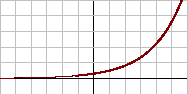
\includegraphics[width=\textwidth]{tex/images/activation/softmax}
    \end{minipage} & -  & -\\
    
% Maxout & \begin{minipage}{.2\textwidth}
%       \includegraphics[width=\textwidth]{example-image-a}
%     \end{minipage} & - & - & - \\
    
\hline

\end{tabular}

\section{loss}
\section{gradient descend + backprop}
\section{ANN}
\section{FeedForward}
\section{DeepNN}
\section{other ML models}

As this thesis focuses mostly on NN, we will just mention other used models.



